Make a simple, interactive program using the Canvas library, and which could be the start of a game. You are to modify the demo-program \lstinline[language=console]{color_boxes.fsx}, such that instead of colored boxes the resulting program:
\begin{enumerate}
\item Creates an interactive canvas
\item Draws a black box on a white background with grey lines from the corners of the box to the nearest corner of the canvas-
\item When the user presses the right or left arror key, then the box with lines are moved to the right and left respectively.
\end{enumerate}
An example of how this could look is:\\
\begin{minipage}{\linewidth}
  \centering
  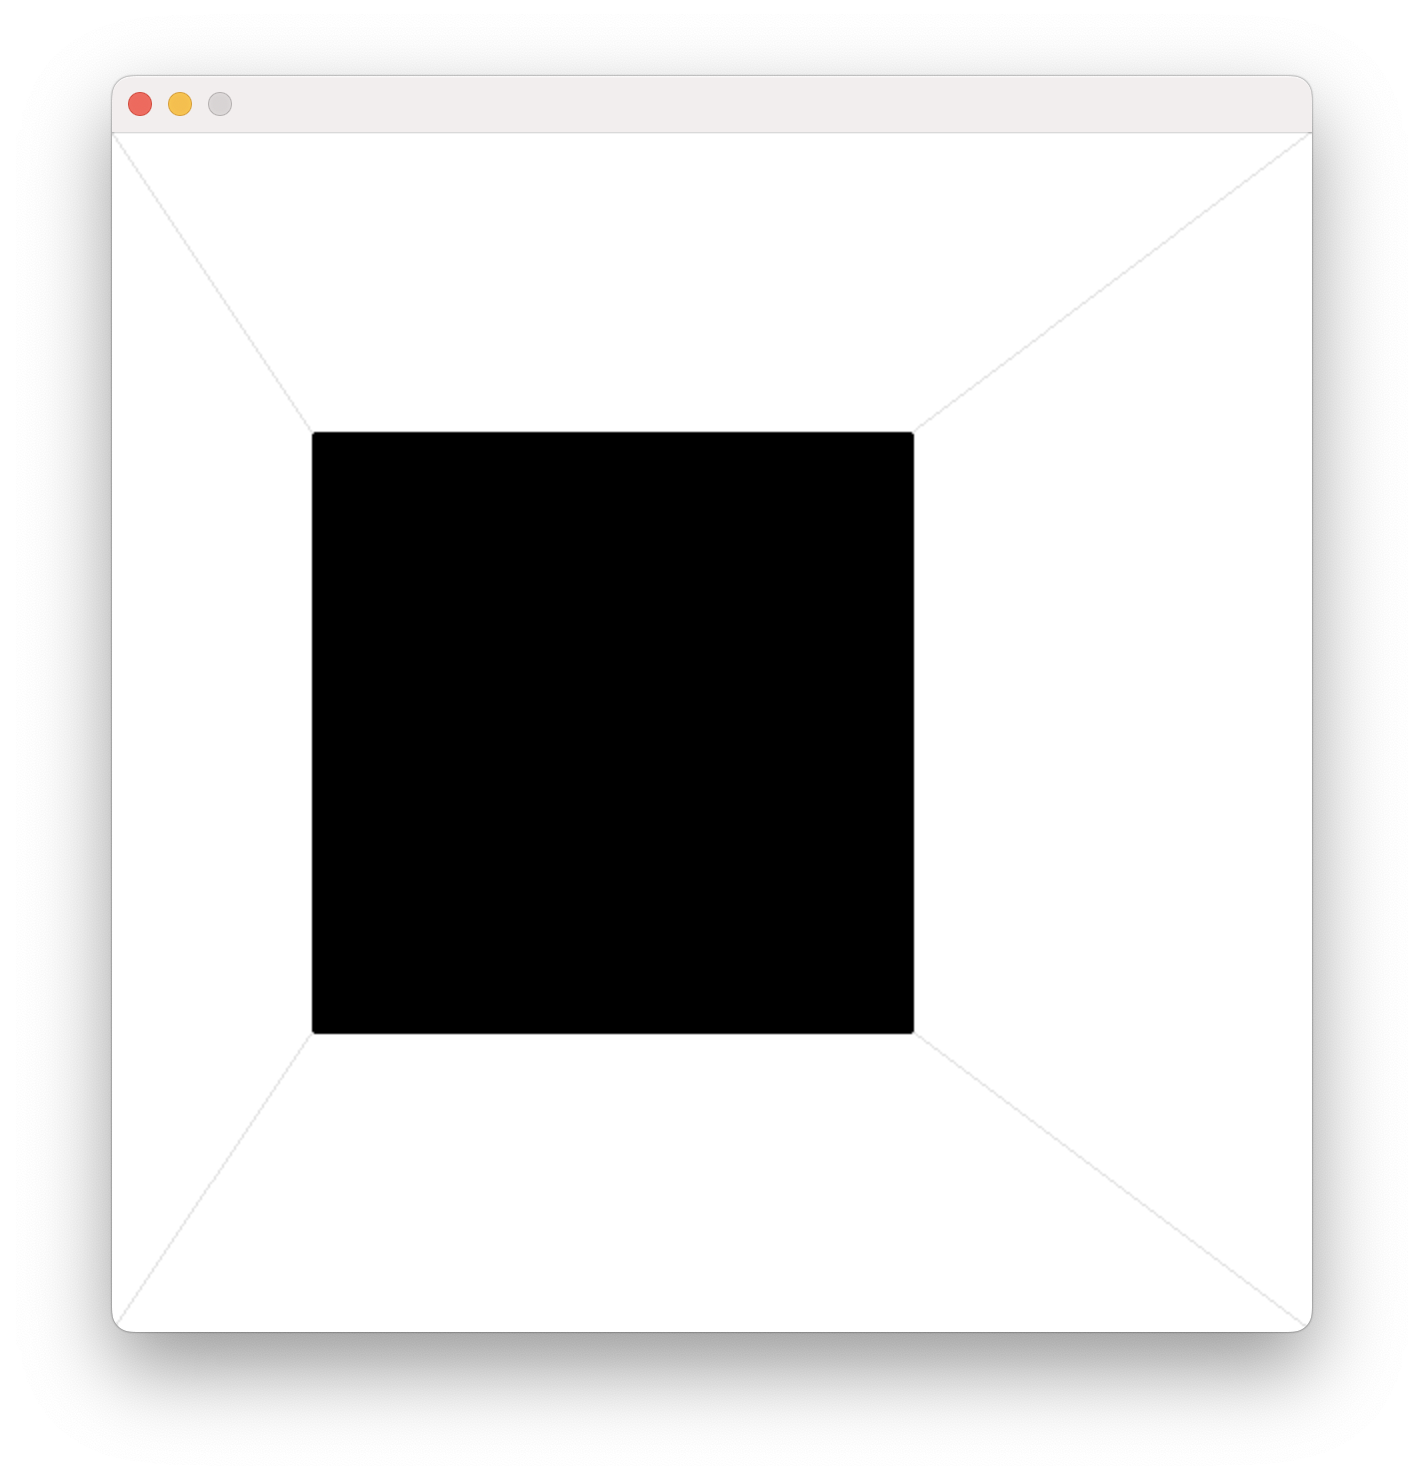
\includegraphics[width=0.6\linewidth]{theBox}
\end{minipage}\\
The functions \lstinline{runApp}, \lstinline{setLine}, and \lstinline{getKey} are most likely essential for this task.

%Du skal kort beskrive din løsning i LaTeX vha.\ \lstinline[language=console]{opgave.tex} skabelonen, og afleveringen skal som minimum indeholde et screen-shot af dit Canvas vinduet
